\newpage
\section*{Part C: Exercise 10.2}

\textit{In Q.1 to 3, choose the correct option and give justification.}

%---------------------------------------------------------------
\subsection*{Exercise 10.2, Question 1}
\textbf{Question.} From a point $Q$, the length of the tangent to a circle is $24$ cm and the distance of $Q$ from the centre is $25$ cm. The radius of the circle is\\
(A) $7$ cm \qquad (B) $12$ cm \qquad (C) $15$ cm \qquad (D) $24.5$ cm

\begin{center}
\begin{tikzpicture}[scale=0.2]
\coordinate (O) at (0,0); \coordinate (Q) at (25,0);
\coordinate (P) at ({49/25},{168/25});
\draw (O) circle (7);
\draw (P) -- (Q); \draw[dashed] (O) -- (P); \draw (O) -- (Q);
\draw pic[draw,angle radius=0.3cm] {right angle=O--P--Q};
\dotat{O}{left}\dotat{P}{above}\dotat{Q}{right}
\node[font=\small,below] at (12.5,0) {$25$ cm};
\node[font=\small,above right] at (13.5,3.3) {$24$ cm};
\end{tikzpicture}%
\figcap{$QP$ is the tangent from $Q$, $P$ the point of contact, $O$ the centre. Dashed line: construction.}
\end{center}

\textbf{Solution.} Let the tangent from $Q$ touch the circle at $P$, so $QP=24$ cm and $OQ=25$ cm. Join $OP$; it is the radius $r$.

The tangent is perpendicular to the radius through the point of contact, so $\ang OPQ=90\deg$. In the right triangle $OPQ$, by the Pythagoras theorem $OQ^2=OP^2+PQ^2$:
\begin{align*}
OP^2&=OQ^2-PQ^2\\
&=25^2-24^2\\
&=625-576=49\\
OP&=\sqrt{49}=7\text{ cm}.
\end{align*}
\slip{The right angle is at $P$ (where the tangent meets the radius), so the hypotenuse is $OQ=25$, the distance from the centre. The radius is a \emph{leg}. Using $OP^2=25^2+24^2$ would treat the radius as the hypotenuse, which is wrong.}

\textbf{Verification.} $OP^2+PQ^2=7^2+24^2=49+576=625=25^2=OQ^2$.

\ans{Option (A): the radius is $7$ cm.}

%---------------------------------------------------------------
\Needspace{26\baselineskip}
\subsection*{Exercise 10.2, Question 2}
\textbf{Question.} In Fig.\ 10.11, if $TP$ and $TQ$ are the two tangents to a circle with centre $O$ so that $\ang POQ=110\deg$, then $\ang PTQ$ is equal to\\
(A) $60\deg$ \qquad (B) $70\deg$ \qquad (C) $80\deg$ \qquad (D) $90\deg$

\begin{center}
\begin{tikzpicture}[scale=1]
\coordinate (O) at (0,0); \coordinate (Q) at (2,0);
\coordinate (P) at (110:2);
\coordinate (T) at (2,{2*tan(55)});
\draw (O) circle (2);
\draw (T) -- (P); \draw (T) -- (Q); \draw (O) -- (P); \draw (O) -- (Q);
\draw pic["$110\deg$",draw,angle radius=0.55cm,angle eccentricity=1.55,font=\scriptsize] {angle=Q--O--P};
\draw pic[draw,angle radius=0.25cm] {right angle=O--P--T};
\draw pic[draw,angle radius=0.25cm] {right angle=T--Q--O};
\dotat{O}{below left}\dotat{P}{above left}\dotat{Q}{below right}\dotat{T}{above right}
\end{tikzpicture}%
\figcap{Fig.\ 10.11 (redrawn).}
\end{center}

\textbf{Solution.} $TP$ and $TQ$ are tangents, so each is perpendicular to the radius through its point of contact (the tangent is perpendicular to the radius at the point of contact):
\[\ang OPT=90\deg,\qquad \ang OQT=90\deg.\]
The angles of the quadrilateral $OPTQ$ add up to $360\deg$:
\begin{align*}
\ang OPT+\ang PTQ+\ang OQT+\ang POQ&=360\deg\\
90\deg+\ang PTQ+90\deg+110\deg&=360\deg\\
\ang PTQ&=360\deg-290\deg=70\deg.
\end{align*}
Here $90\deg+90\deg+110\deg=290\deg$.
\slip{The four angles of $OPTQ$ are the two right angles at $P$ and $Q$, the given $\ang POQ=110\deg$, and the unknown $\ang PTQ$. A common slip is to use $180\deg$ (triangle sum) instead of $360\deg$ (quadrilateral sum).}

\textbf{Verification.} $\ang PTQ+\ang POQ=70\deg+110\deg=180\deg$, which agrees with the result of Question 10 (the angle between the tangents and the angle at the centre are supplementary).

\ans{Option (B): $\ang PTQ=70\deg$.}

%---------------------------------------------------------------
\subsection*{Exercise 10.2, Question 3}
\textbf{Question.} If tangents $PA$ and $PB$ from a point $P$ to a circle with centre $O$ are inclined to each other at angle of $80\deg$, then $\ang POA$ is equal to\\
(A) $50\deg$ \qquad (B) $60\deg$ \qquad (C) $70\deg$ \qquad (D) $80\deg$

\begin{center}
\begin{tikzpicture}[scale=1]
\coordinate (O) at (0,0); \coordinate (P) at ({-2/sin(40)},0);
\coordinate (A) at (130:2); \coordinate (B) at (230:2);
\draw (O) circle (2);
\draw (P) -- (A); \draw (P) -- (B); \draw (O) -- (A); \draw (O) -- (B); \draw[dashed] (O) -- (P);
\draw pic[draw,angle radius=0.9cm] {angle=B--P--A};
\draw pic[draw,angle radius=0.25cm] {right angle=P--A--O};
\draw pic[draw,angle radius=0.25cm] {right angle=O--B--P};
\node[font=\scriptsize,above] at ($(P)+(1.35,0)$) {$80\deg$};
\dotat{O}{right}\dotat{P}{left}\dotat{A}{above}\dotat{B}{below}
\end{tikzpicture}%
\figcap{Tangents $PA$ and $PB$; dashed line: construction $OP$.}
\end{center}

\textbf{Solution.} The tangent is perpendicular to the radius through the point of contact, so $\ang OAP=\ang OBP=90\deg$.

In $\tri OAP$ and $\tri OBP$: $OA=OB$ (radii), $OP$ is common, and $\ang OAP=\ang OBP=90\deg$. So $\tri OAP\cong\tri OBP$ (RHS) and $\ang OPA=\ang OPB$ (CPCT). Therefore $OP$ bisects $\ang APB$:
\[\ang OPA=\tfrac12\times 80\deg=40\deg.\]
In $\tri OAP$, by the angle-sum property,
\[\ang POA=180\deg-\ang OAP-\ang OPA=180\deg-90\deg-40\deg=50\deg.\]
\slip{The $80\deg$ is the angle $\ang APB$ \emph{between the tangents}, not $\ang POA$. The line $OP$ cuts it into two halves of $40\deg$. Answering $80\deg$ (option D) confuses that angle with $\ang POA$; stopping at $\ang OPA=40\deg$ forgets the final angle-sum step in $\tri OAP$.}

\textbf{Verification.} By Question 10, $\ang AOB=180\deg-80\deg=100\deg$, and $OP$ bisects it, so $\ang POA=\tfrac12\times100\deg=50\deg$.

\ans{Option (A): $\ang POA=50\deg$.}

%---------------------------------------------------------------
\subsection*{Exercise 10.2, Question 4}
\textbf{Question.} Prove that the tangents drawn at the ends of a diameter of a circle are parallel.

\begin{center}
\begin{tikzpicture}[scale=1]
\coordinate (O) at (0,0); \coordinate (A) at (-2,0); \coordinate (B) at (2,0);
\draw (O) circle (2);
\draw (-2,-2.7) -- (-2,2.7); \draw (2,-2.7) -- (2,2.7);
\draw (A) -- (B);
\dotat{O}{above}\dotat{A}{above left}\dotat{B}{above right}
\node[above left] at (-2,2.7) {$P$}; \node[below left] at (-2,-2.7) {$Q$};
\node[above right] at (2,2.7) {$R$}; \node[below right] at (2,-2.7) {$S$};
\end{tikzpicture}%
\figcap{$AB$ is a diameter; $PQ$ and $RS$ are the tangents at $A$ and $B$.}
\end{center}

\textbf{Solution.}

\textbf{Given:} A circle with centre $O$ and diameter $AB$. $PQ$ is the tangent at $A$ and $RS$ is the tangent at $B$, with $P$ and $R$ on the same side of $AB$.

\textbf{To prove:} $PQ\parallel RS$.

\proofhd{}
\begin{prf}
1 & $\ang PAB=90\deg$. & The tangent at $A$ is perpendicular to the radius $OA$, and $OA$ lies along the diameter $AB$. \\
2 & $\ang ABS=90\deg$. & The tangent at $B$ is perpendicular to the radius $OB$, and $OB$ lies along $AB$. \\
3 & $\ang PAB=\ang ABS$. & Each is $90\deg$ (steps 1 and 2). \\
4 & These are alternate interior angles formed by the lines $PQ$ and $RS$ with the transversal $AB$. & $P$ and $S$ lie on opposite sides of $AB$. \\
5 & $PQ\parallel RS$. & If a transversal makes equal alternate interior angles with two lines, the lines are parallel.
\end{prf}

\ans{The tangents at the ends of a diameter are parallel. (Proved)}

%---------------------------------------------------------------
\subsection*{Exercise 10.2, Question 5}
\textbf{Question.} Prove that the perpendicular at the point of contact to the tangent to a circle passes through the centre.

\begin{center}
\begin{tikzpicture}[scale=1]
\coordinate (O) at (0,0); \coordinate (P) at (0,-2);
\draw (O) circle (2);
\draw (-3,-2) -- (3,-2);
\dotat{O}{right}\dotat{P}{below right}
\node[left] at (-3,-2) {$X$}; \node[right] at (3,-2) {$Y$};
\end{tikzpicture}%
\figcap{$XY$ is the tangent at $P$; $O$ is the centre.}
\end{center}

\textbf{Solution.}

\textbf{Given:} A circle with centre $O$ and a tangent $XY$ touching it at $P$. Let $\ell$ be the line through $P$ perpendicular to $XY$.

\textbf{To prove:} $\ell$ passes through $O$.

\textbf{Construction:} Join $OP$.

\proofhd{}
\begin{prf}
1 & $OP\perp XY$. & The tangent is perpendicular to the radius through the point of contact. \\
2 & $\ell\perp XY$ at $P$. & Given. \\
3 & $OP$ and $\ell$ are both perpendicular to $XY$ at the same point $P$. & Steps 1 and 2. \\
4 & $OP$ and $\ell$ are the same line. & Through a given point of a line, only one perpendicular to that line can be drawn. \\
5 & $\ell$ passes through $O$. & $OP$ passes through $O$ (step 4).
\end{prf}

\ans{The perpendicular to a tangent at the point of contact passes through the centre of the circle. (Proved)}

%---------------------------------------------------------------
\subsection*{Exercise 10.2, Question 6}
\textbf{Question.} The length of a tangent from a point $A$ at distance $5$ cm from the centre of the circle is $4$ cm. Find the radius of the circle.

\begin{center}
\begin{tikzpicture}[scale=0.55]
\coordinate (O) at (0,0); \coordinate (A) at (5,0);
\coordinate (P) at ({9/5},{12/5});
\draw (O) circle (3);
\draw (A) -- (P); \draw[dashed] (O) -- (P); \draw (O) -- (A);
\draw pic[draw,angle radius=0.3cm] {right angle=O--P--A};
\dotat{O}{left}\dotat{P}{above}\dotat{A}{right}
\node[font=\small,below] at (4.1,0) {$5$ cm};
\node[font=\small,above right] at (3.5,1.3) {$4$ cm};
\end{tikzpicture}%
\figcap{$AP$ is the tangent from $A$ with point of contact $P$. Dashed line: construction.}
\end{center}

\textbf{Solution.} Let the tangent from $A$ touch the circle at $P$, so $AP=4$ cm and $OA=5$ cm. Join $OP$; it is the radius $r$.

The tangent is perpendicular to the radius through the point of contact, so $\ang OPA=90\deg$. By the Pythagoras theorem in $\tri OPA$, $OA^2=OP^2+AP^2$:
\begin{align*}
OP^2&=OA^2-AP^2\\
&=5^2-4^2\\
&=25-16=9\\
OP&=\sqrt9=3\text{ cm}.
\end{align*}
\slip{The distance $OA=5$ cm from the centre is the hypotenuse (opposite the right angle at $P$), and the tangent length $AP=4$ cm and the radius are the legs. So subtract: $5^2-4^2$, not $5^2+4^2$.}

\textbf{Verification.} $OP^2+AP^2=3^2+4^2=9+16=25=5^2=OA^2$.

\ans{The radius of the circle is $3$ cm.}

%---------------------------------------------------------------
\Needspace{26\baselineskip}
\subsection*{Exercise 10.2, Question 7}
\textbf{Question.} Two concentric circles are of radii $5$ cm and $3$ cm. Find the length of the chord of the larger circle which touches the smaller circle.

\begin{center}
\begin{tikzpicture}[scale=0.6]
\coordinate (O) at (0,0);
\draw (O) circle (5); \draw (O) circle (3);
\coordinate (P) at (-50:3);
\coordinate (A) at ($(P)+(40:4)$); \coordinate (B) at ($(P)-(40:4)$);
\draw (A) -- (B); \draw[dashed] (O) -- (P); \draw[dashed] (O) -- (A);
\draw pic[draw,angle radius=0.3cm] {right angle=A--P--O};
\dotat{O}{above left}\dotat{P}{below right}\dotat{A}{above right}\dotat{B}{below}
\node[font=\small,left] at ($(O)!0.5!(P)$) {$3$ cm};
\node[font=\small,above] at ($(O)!0.8!(A)$) {$5$ cm};
\end{tikzpicture}%
\figcap{Chord $AB$ of the larger circle touches the smaller circle at $P$. Dashed lines: construction.}
\end{center}

\textbf{Solution.} Let $AB$ be the chord of the larger circle (radius $5$ cm) that touches the smaller circle (radius $3$ cm) at $P$. Join $OP$ and $OA$, so $OP=3$ cm and $OA=5$ cm.

$AB$ is a tangent to the smaller circle at $P$, so $OP\perp AB$ (the tangent is perpendicular to the radius through the point of contact). In the right triangle $OPA$, by the Pythagoras theorem $OA^2=OP^2+AP^2$:
\begin{align*}
AP^2&=OA^2-OP^2\\
&=5^2-3^2\\
&=25-9=16\\
AP&=\sqrt{16}=4\text{ cm}.
\end{align*}
$OP$ is the perpendicular from the centre $O$ to the chord $AB$ of the larger circle, so it bisects the chord (the perpendicular from the centre of a circle to a chord bisects the chord; see Example 1). Hence $AB=2\times AP=2\times4=8$ cm.
\slip{$AP=4$ cm is only \emph{half} the chord. The question asks for the whole chord $AB$, so the last step $2\times4$ must not be left out.}

\textbf{Verification.} Half-chord $AP=4$, so $AP^2+OP^2=4^2+3^2=16+9=25=5^2=OA^2$.

\ans{The length of the chord is $8$ cm.}

%---------------------------------------------------------------
\subsection*{Exercise 10.2, Question 8}
\textbf{Question.} A quadrilateral $ABCD$ is drawn to circumscribe a circle (see Fig.\ 10.12). Prove that $AB+CD=AD+BC$.

\begin{center}
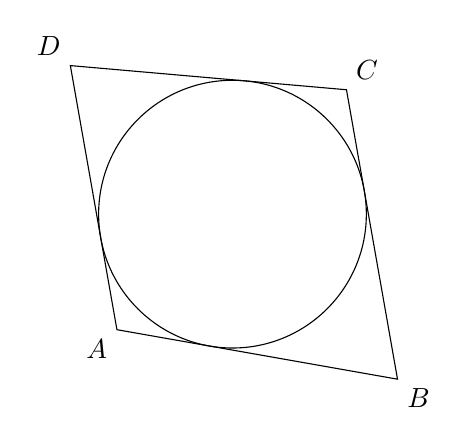
\begin{tikzpicture}[scale=0.85]
\coordinate (O) at (0,0);
\coordinate (A) at (225:{2/cos(35)}); \coordinate (B) at (315:{2/cos(55)});
\coordinate (C) at (47.5:{2/cos(37.5)}); \coordinate (D) at (137.5:{2/cos(52.5)});
\coordinate (P) at (260:2); \coordinate (Q) at (10:2);
\coordinate (R) at (85:2); \coordinate (S) at (190:2);
\draw (O) circle (2);
\draw (A) -- (B) -- (C) -- (D) -- cycle;
\dotat{P}{below}\dotat{Q}{right}\dotat{R}{above}\dotat{S}{left}
\node[below left] at (A) {$A$}; \node[below right] at (B) {$B$};
\node[above right] at (C) {$C$}; \node[above left] at (D) {$D$};
\end{tikzpicture}%
\figcap{Fig.\ 10.12 (redrawn). $P,Q,R,S$ are the points of contact on $AB,BC,CD,DA$.}
\end{center}

\textbf{Solution.}

\textbf{Given:} A quadrilateral $ABCD$ whose sides $AB$, $BC$, $CD$, $DA$ touch a circle at $P$, $Q$, $R$, $S$ respectively.

\textbf{To prove:} $AB+CD=AD+BC$.

\proofhd{}
\begin{prf}
1 & $AP=AS$ & Tangents from the external point $A$ are equal. \\
2 & $BP=BQ$ & Tangents from the external point $B$ are equal. \\
3 & $CR=CQ$ & Tangents from the external point $C$ are equal. \\
4 & $DR=DS$ & Tangents from the external point $D$ are equal. \\
5 & $AP+BP+CR+DR=AS+BQ+CQ+DS$ & Adding steps 1 to 4. \\
6 & $(AP+BP)+(CR+DR)=(AS+DS)+(BQ+CQ)$ & Regrouping step 5. \\
7 & $AB+CD=AD+BC$ & $P$ lies on $AB$, $R$ on $CD$, $S$ on $DA$, $Q$ on $BC$, so $AP+BP=AB$, $CR+DR=CD$, $AS+DS=AD$, $BQ+CQ=BC$.
\end{prf}

\ans{$AB+CD=AD+BC$. (Proved)}

%---------------------------------------------------------------
\subsection*{Exercise 10.2, Question 9}
\textbf{Question.} In Fig.\ 10.13, $XY$ and $X'Y'$ are two parallel tangents to a circle with centre $O$ and another tangent $AB$ with point of contact $C$ intersecting $XY$ at $A$ and $X'Y'$ at $B$. Prove that $\ang AOB=90\deg$.

\begin{center}
\begin{tikzpicture}[scale=1]
\coordinate (O) at (0,0); \coordinate (P) at (0,2); \coordinate (Q) at (0,-2);
\coordinate (C) at (-20:2);
\coordinate (A) at ({(2-2*sin(-20))/cos(-20)},2);
\coordinate (B) at ({(2+2*sin(-20))/cos(-20)},-2);
\draw (O) circle (2);
\draw (-3,2) -- (4.2,2); \draw (-3,-2) -- (4.2,-2);
\draw (A) -- (B);
\draw[dashed] (O) -- (P); \draw[dashed] (O) -- (Q); \draw[dashed] (O) -- (C);
\draw[dashed] (O) -- (A); \draw[dashed] (O) -- (B);
\dotat{O}{left}\dotat{P}{above left}\dotat{Q}{below left}\dotat{C}{right}
\node[above right] at (A) {$A$}; \node[below right] at (B) {$B$};
\node[left] at (-3,2) {$X$}; \node[right] at (4.2,2) {$Y$};
\node[left] at (-3,-2) {$X'$}; \node[right] at (4.2,-2) {$Y'$};
\end{tikzpicture}%
\figcap{Fig.\ 10.13 (redrawn). $P$ and $Q$ are the points of contact of $XY$ and $X'Y'$. Dashed lines: construction.}
\end{center}

\textbf{Solution.}

\textbf{Given:} $XY\parallel X'Y'$ are tangents to a circle with centre $O$, touching it at $P$ and $Q$. The tangent $AB$ touches the circle at $C$ and meets $XY$ at $A$ and $X'Y'$ at $B$.

\textbf{To prove:} $\ang AOB=90\deg$.

\textbf{Construction:} Join $OP$, $OQ$, $OC$, $OA$ and $OB$.

\proofhd{}
\begin{prf}
1 & $\ang OPA=\ang OCA=90\deg$. & The tangent is perpendicular to the radius through the point of contact. \\
2 & In $\tri OPA$ and $\tri OCA$: $OP=OC$, $OA$ is common and $\ang OPA=\ang OCA=90\deg$. So $\tri OPA\cong\tri OCA$. & $OP$, $OC$ are radii; RHS congruence. \\
3 & $\ang OAP=\ang OAC$, so $\ang PAB=2\ang OAB$. & CPCT; $C$ lies on $AB$, so $\ang OAC=\ang OAB$ and $\ang PAC=\ang PAB$. \\
4 & Similarly $\tri OQB\cong\tri OCB$, so $\ang QBA=2\ang OBA$. & Same reasoning at $B$ (RHS, then CPCT). \\
5 & $\ang PAB+\ang QBA=180\deg$. & Interior angles on the same side of the transversal $AB$ for the parallel lines $XY$ and $X'Y'$. \\
6 & $2\ang OAB+2\ang OBA=180\deg$, so $\ang OAB+\ang OBA=90\deg$. & Steps 3, 4 and 5. \\
7 & $\ang AOB=180\deg-(\ang OAB+\ang OBA)=90\deg$. & Angle-sum property of $\tri AOB$.
\end{prf}

\slip{Step 3 says $\ang PAB=2\ang OAB$, not $\ang PAB=\ang OAB$: $AO$ bisects the angle $\ang PAB$ because the two triangles at $A$ are congruent. Forgetting the factor $2$ makes step 6 give $\ang OAB+\ang OBA=180\deg$, which is wrong.}

\ans{$\ang AOB=90\deg$. (Proved)}

\textbf{Alternative proof.} Join $OP,OQ,OC$. By RHS, $\tri OPA\cong\tri OCA$ and $\tri OQB\cong\tri OCB$, so $\ang AOP=\ang AOC$ and $\ang BOQ=\ang BOC$. Since $XY\parallel X'Y'$, both $OP$ and $OQ$ are perpendicular to $X'Y'$ through $O$, so $POQ$ is a straight line and $\ang POQ=180\deg$. Then $\ang AOP+\ang AOC+\ang BOC+\ang BOQ=180\deg$, i.e. $2(\ang AOC+\ang BOC)=180\deg$, so $\ang AOB=\ang AOC+\ang BOC=90\deg$.

%---------------------------------------------------------------
\subsection*{Exercise 10.2, Question 10}
\textbf{Question.} Prove that the angle between the two tangents drawn from an external point to a circle is supplementary to the angle subtended by the line-segment joining the points of contact at the centre.

\begin{center}
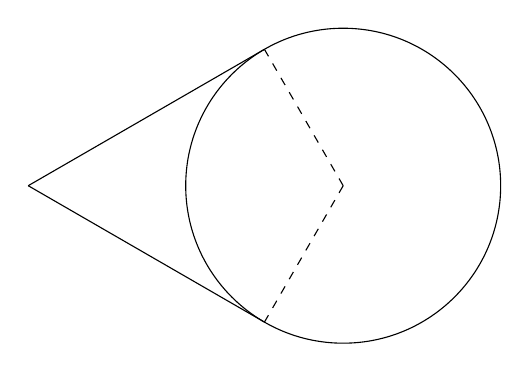
\begin{tikzpicture}[scale=1]
\coordinate (O) at (0,0); \coordinate (P) at (-4,0);
\coordinate (A) at (120:2); \coordinate (B) at (240:2);
\draw (O) circle (2);
\draw (P) -- (A); \draw (P) -- (B); \draw[dashed] (O) -- (A); \draw[dashed] (O) -- (B);
\dotat{O}{right}\dotat{P}{left}\dotat{A}{above}\dotat{B}{below}
\end{tikzpicture}%
\figcap{$PA$ and $PB$ are tangents from $P$; $A$ and $B$ are the points of contact. Dashed lines: construction.}
\end{center}

\textbf{Solution.}

\textbf{Given:} A circle with centre $O$; an external point $P$; tangents $PA$ and $PB$ touching the circle at $A$ and $B$.

\textbf{To prove:} $\ang APB+\ang AOB=180\deg$.

\textbf{Construction:} Join $OA$ and $OB$.

\proofhd{}
\begin{prf}
1 & $\ang OAP=90\deg$ and $\ang OBP=90\deg$. & The tangent is perpendicular to the radius through the point of contact. \\
2 & $\ang OAP+\ang APB+\ang OBP+\ang AOB=360\deg$. & Angle-sum property of the quadrilateral $OAPB$. \\
3 & $90\deg+\ang APB+90\deg+\ang AOB=360\deg$. & Substituting step 1 in step 2. \\
4 & $\ang APB+\ang AOB=180\deg$. & From step 3.
\end{prf}

\ans{The angle between the two tangents and the angle subtended at the centre by the segment joining the points of contact add up to $180\deg$, i.e. they are supplementary. (Proved)}

%---------------------------------------------------------------
\subsection*{Exercise 10.2, Question 11}
\textbf{Question.} Prove that the parallelogram circumscribing a circle is a rhombus.

\textbf{Note on the figure.} No separate figure is drawn: an accurate figure of a parallelogram circumscribing a circle is already a rhombus, so it would show the result. Use the labels of the figure of Question 8 (points of contact $P,Q,R,S$ on $AB,BC,CD,DA$).

\textbf{Solution.}

\textbf{Given:} A parallelogram $ABCD$ whose sides $AB$, $BC$, $CD$, $DA$ touch a circle at $P$, $Q$, $R$, $S$.

\textbf{To prove:} $ABCD$ is a rhombus, i.e. $AB=BC=CD=DA$.

\proofhd{}
\begin{prf}
1 & $AB+CD=AD+BC$. & For a quadrilateral circumscribing a circle, sums of opposite sides are equal (Question 8, which uses ``tangents from an external point are equal''). \\
2 & $AB=CD$ and $AD=BC$. & Opposite sides of a parallelogram are equal. \\
3 & $2AB=2AD$, so $AB=AD$. & Substituting step 2 in step 1. \\
4 & $AB=BC=CD=DA$. & $AB=CD$, $AD=BC$ (step 2) and $AB=AD$ (step 3). \\
5 & $ABCD$ is a rhombus. & A parallelogram with all four sides equal is a rhombus.
\end{prf}

\ans{A parallelogram that circumscribes a circle is a rhombus. (Proved)}

%---------------------------------------------------------------
\subsection*{Exercise 10.2, Question 12}
\textbf{Question.} A triangle $ABC$ is drawn to circumscribe a circle of radius $4$ cm such that the segments $BD$ and $DC$ into which $BC$ is divided by the point of contact $D$ are of lengths $8$ cm and $6$ cm respectively (see Fig.\ 10.14). Find the sides $AB$ and $AC$.

\begin{center}
\begin{tikzpicture}[scale=0.42]
\coordinate (C) at (0,0); \coordinate (B) at (14,0); \coordinate (A) at (5,12);
\coordinate (O) at (6,4); \coordinate (D) at (6,0);
\coordinate (E) at ($(A)!{7/13}!(C)$); \coordinate (F) at ($(A)!{7/15}!(B)$);
\draw (O) circle (4);
\draw (A) -- (B) -- (C) -- cycle;
\draw[dashed] (O) -- (D);
\draw pic[draw,angle radius=0.3cm] {right angle=B--D--O};
\dotat{O}{above}\dotat{D}{below}\dotat{E}{left}\dotat{F}{right}
\node[above] at (A) {$A$}; \node[left] at (C) {$C$}; \node[right] at (B) {$B$};
\node[font=\small,below] at (3,0) {$6$ cm}; \node[font=\small,below] at (10,0) {$8$ cm};
\node[font=\small,right] at (6,2) {$4$ cm};
\end{tikzpicture}%
\figcap{Fig.\ 10.14 (redrawn). The circle touches $BC$, $CA$, $AB$ at $D$, $E$, $F$.}
\end{center}

\textbf{Solution.} Let the circle touch $BC$, $CA$, $AB$ at $D$, $E$, $F$ respectively, and let $AE=AF=x$ cm.

\textbf{Step 1: express the sides using equal tangents} (tangents from an external point are equal):
\begin{align*}
BF&=BD=8\text{ cm}, & CE&=CD=6\text{ cm}, & AF&=AE=x\text{ cm},\\
AB&=AF+FB=(x+8)\text{ cm}, & AC&=AE+EC=(x+6)\text{ cm}, & BC&=BD+DC=14\text{ cm}.
\end{align*}

\textbf{Step 2: area by Heron's formula.} For sides $a,b,c$ and $s=\dfrac{a+b+c}{2}$,
\[\text{area}=\sqrt{s(s-a)(s-b)(s-c)}.\]
Take $a=BC=14$, $b=CA=x+6$, $c=AB=x+8$:
\[s=\frac{14+(x+6)+(x+8)}{2}=x+14,\quad s-a=x,\quad s-b=8,\quad s-c=6.\]
\[\text{ar}(\tri ABC)=\sqrt{(x+14)\cdot x\cdot 8\cdot 6}=\sqrt{48x(x+14)}.\]

\textbf{Step 3: area using the radius.} Join $O$ to $A$, $B$, $C$. The triangle $ABC$ splits into $\tri OBC$, $\tri OCA$, $\tri OAB$. Each has height equal to the radius $r=4$ cm, because the radius to a point of contact is perpendicular to the tangent. Area of a triangle with inradius $r$ is $\tfrac12\times r\times\text{perimeter}$:
\[\text{ar}(\tri ABC)=\tfrac12\times4\times\big(14+(x+6)+(x+8)\big)=\tfrac12\times4\times(2x+28)=4(x+14).\]

\textbf{Step 4: equate and solve.} Both expressions are the area of $\tri ABC$:
\begin{align*}
\sqrt{48x(x+14)}&=4(x+14)\\
48x(x+14)&=\big(4(x+14)\big)^2=16(x+14)^2 &&\text{(squaring both sides)}\\
\frac{48x(x+14)}{16(x+14)}&=\frac{16(x+14)^2}{16(x+14)} &&\text{(dividing both sides by }16(x+14)\neq0\text{)}\\
3x&=x+14 &&\text{(}48\div16=3\text{ and }(x+14)^2\div(x+14)=x+14\text{)}\\
3x-x&=14\\
2x&=14\\
x&=7.
\end{align*}
Therefore, putting $x=7$: $AB=x+8=7+8=15$ cm and $AC=x+6=7+6=13$ cm.
\slip{In Step 4 the factor $(x+14)$ appears on both sides, so dividing by it is allowed only because $x+14\neq0$ (lengths are positive). Also, $AB=x+8$ and $AC=x+6$: the $8$ goes with $B$ and the $6$ with $C$, because $BD=8$ and $CD=6$.}

\textbf{Verification.} The sides are $AB=15$, $AC=13$, $BC=14$, so $s=\dfrac{15+13+14}{2}=21$. By Heron's formula:
\[\text{area}=\sqrt{21\cdot(21-14)(21-13)(21-15)}=\sqrt{21\cdot7\cdot8\cdot6}=\sqrt{7056}=84.\]
By the inradius formula: $\tfrac12\times4\times(15+13+14)=\tfrac12\times4\times42=84$. The two areas agree.

\ans{$AB=15$ cm and $AC=13$ cm.}

%---------------------------------------------------------------
\subsection*{Exercise 10.2, Question 13}
\textbf{Question.} Prove that opposite sides of a quadrilateral circumscribing a circle subtend supplementary angles at the centre of the circle.

\begin{center}
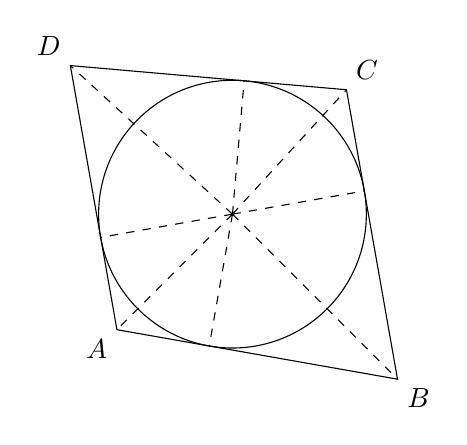
\begin{tikzpicture}[scale=0.85]
\coordinate (O) at (0,0);
\coordinate (A) at (225:{2/cos(35)}); \coordinate (B) at (315:{2/cos(55)});
\coordinate (C) at (47.5:{2/cos(37.5)}); \coordinate (D) at (137.5:{2/cos(52.5)});
\coordinate (P) at (260:2); \coordinate (Q) at (10:2);
\coordinate (R) at (85:2); \coordinate (S) at (190:2);
\draw (O) circle (2);
\draw (A) -- (B) -- (C) -- (D) -- cycle;
\foreach \v in {A,B,C,D,P,Q,R,S}{\draw[dashed] (O) -- (\v);}
\dotat{O}{above right}\dotat{P}{below}\dotat{Q}{right}\dotat{R}{above}\dotat{S}{left}
\node[below left] at (A) {$A$}; \node[below right] at (B) {$B$};
\node[above right] at (C) {$C$}; \node[above left] at (D) {$D$};
\end{tikzpicture}%
\figcap{$ABCD$ circumscribes the circle with centre $O$; $P,Q,R,S$ are the points of contact. Dashed lines: construction.}
\end{center}

\textbf{Solution.}

\textbf{Given:} A quadrilateral $ABCD$ circumscribing a circle with centre $O$; the sides $AB$, $BC$, $CD$, $DA$ touch the circle at $P$, $Q$, $R$, $S$.

\textbf{To prove:} $\ang AOB+\ang COD=180\deg$ and $\ang AOD+\ang BOC=180\deg$.

\textbf{Construction:} Join $OA$, $OB$, $OC$, $OD$, $OP$, $OQ$, $OR$, $OS$.

\proofhd{}
\begin{prf}
1 & $\ang OPA=\ang OSA=90\deg$. & The tangent is perpendicular to the radius through the point of contact. \\
2 & In $\tri OPA$ and $\tri OSA$: $OP=OS$, $OA$ is common, $\ang OPA=\ang OSA=90\deg$. So $\tri OPA\cong\tri OSA$. & $OP$, $OS$ are radii; RHS congruence. \\
3 & $\ang AOP=\ang AOS$. Call each $a$. & CPCT. \\
4 & In the same way, $\ang BOP=\ang BOQ=b$, $\ang COQ=\ang COR=c$, $\ang DOR=\ang DOS=d$. & RHS and CPCT at $B$, $C$, $D$. \\
5 & $2a+2b+2c+2d=360\deg$, so $a+b+c+d=180\deg$. & The angles around the point $O$ add up to $360\deg$. \\
6 & $\ang AOB=a+b$, $\ang COD=c+d$, $\ang AOD=a+d$, $\ang BOC=b+c$. & $OP$ lies inside $\ang AOB$, $OQ$ inside $\ang BOC$, $OR$ inside $\ang COD$, $OS$ inside $\ang DOA$. \\
7 & $\ang AOB+\ang COD=(a+b)+(c+d)=180\deg$. & Steps 5 and 6. \\
8 & $\ang AOD+\ang BOC=(a+d)+(b+c)=180\deg$. & Steps 5 and 6.
\end{prf}

\ans{Opposite sides $AB$, $CD$ subtend supplementary angles at $O$, and so do $AD$, $BC$. (Proved)}
